\documentclass[11pt]{article}
\usepackage{sectsty}
\usepackage{hyperref}
\usepackage{graphicx}
\graphicspath{ {images/} }

\sectionfont{\fontsize{10}{10}\selectfont}
\subsectionfont{\fontsize{10}{10}\selectfont}

\begin{document}

\title{Master Thesis - Project Plan}
\author{Dylan Bartels - 10607072\\University of Amsterdam \\dylan.bartels@student.uva.nl}
\maketitle

The following project plan is meant for coordinators around the project to be informed about the general direction of the master thesis project. The current state of the documentation is that of a draft.

\section{Host Organisation}
% Host organization and group: Give pointers (URL, address, documents) to a specific group in the organization that will host this project.
Collaboration got initiated between Dylan Bartels and Hjalmar van der Schaaf during the UvA 2017 thesis fair. CargoLedger is located in the ACE Incubator of the University of Amsterdam. More information regarding CargoLedger can be found on: \url{www.cargoledger.nl}

% Contact person: Give name, function, phone number and e-mail address of the contact person for this project in the host organization.
\subsection*{Contact person: }

Name: \hspace{16mm} drs. Hjalmar van der Schaaf \newline
Function: \hspace{11mm} CEO\newline
Phone Number: \hspace{0.5mm} +31(0)6-21523527\newline
E-mail: \hspace{15mm} hjalmar@headon.nl \newline

% Project summary: Give a short (at most 1 page) description of the project. Make sure that the following issues are covered:
\section{Project Summary}

% The global context of the project,
Cargoledger wants to know how a trustless decentralized peer-to-peer marketplace could support the supply chain. They recently developed the technique of broadcasting smart contracts, representing supply chain goods, on the Ethereum network\cite{buterin2014next}. With this foundation they are aiming to create a marketplace for logistical smart contracts. On this marketplace different actors can broadcast, contribute or fulfill these smart contracts, whereby the smart contract is defined as a request of transport of goods along the supply chain. \par
To put this project into the global context, the values of the project align with reducing centralization, advance transparency and achieving sustainability. Research in the direction could achieve the academic information to build a marketplace whereby individuals can benefit from transporting goods on their everyday transport route. Current transport of goods is done by central entities being a custodian for the transport and bulking the goods from central drop-off points to sorting centers to the actual endpoint. If this transport is open to the public in a peer-to-peer manner the positive benefits can be efficiency and equal opportunities for different size actors.\par

% The relevancy of your research,
Recent successful technical innovations have been due to a shift from centralization to peer-to-peer services, examples of these are Uber, Airbnb and Kickstarter. In the domain of supply chain logistics this innovation has been lacking. Recent research \cite{peer-to-peerDecentralizedLogistics} have proposed a peer-to-peer framework supporting interoperability between different actors in the logistics chains. This research lacks insight related to trust, network and technical implementation but establishes interest in the domain regarding implementation. \par
With the recent progression in the domain of trustless value transference, research towards the applicability of this in the supply chain offers relevancy. In \cite{trustlessIntermediationInBCServiceMarket} research has formulated possible implementation of trustless intermediation in blockchain based decentralized service marketplaces. The research topic arises if this or other intermediation solutions can also be applied to peer-to-peer logistics marketplaces and to which degree will there be a custodian in the process due to it including a physical process. 
% The specific research questions to be answered in the project.
\bigbreak
\noindent Main research question: 
\begin{itemize}
  \item What are the specific problems and characteristics of a trustless decentralized peer-to-peer marketplace for transportation of goods?
\end{itemize}
\bigbreak
\noindent Subquestions: 
\bigbreak 
\noindent For the following subquestions marketplace is defined as a trustless decentralized peer-to-peer marketplace for transportation of goods.
\begin{itemize}
  \item Can trustless intermediation exists on this marketplace without a custodian for dispute prevention and resolution?
  %\item Which strategies can prevent sybil attacks on this marketplace?
  \item What level of anonymity is possible on this marketplace? 
\end{itemize}

% Problem analysis: Here you present your analysis of the problem situation that your research will address. 
\section{Problem analysis}

% How does this problem manifest itself at your host organization?
Cargoledger has been working to integrate the possibility of decentralization throughout the supply chain, what they have not researched is how to connect the demand and supply of the transport. The problem of connecting these two parties is of high importance to open up the supply chain to peer-to-peer possibilities. Research into what the problems and characteristics of such a marketplace are would possibly open the way to such a marketplace and align it with the other product in the company so that a pilot of the full system can be initiated. \par
% Also summarizes existing scientific insight into the problem (result of your literature survey, see below).
% p2p
Peer-to-peer computing \cite{peer2peer} has lead the way for many different applications. Marketplaces have been a domain of research along academia of applying this architecture. In \cite{buildingp2pmarketplace} Ferreira \& Ferreira, 2004 discuss the implementation of essential services for peer-to-peer marketplaces and illustrate its benefits for a vendor. Recent study \cite{challangeDecentralizedMarketplaces}\cite{decentralMarket} has contributed to an distributed permission system, called Dispersy, which simplifies the design of distributed communities. Researchers are able to take this foundation and bootstrap distributed communities and expand it to other domains.\par
A well established peer-to-peer marketplace is Openbazaar. This open-source project has been created in 2014 and has contributed to academic research in the domain\cite{openbazaar}. Openbazaar uses a shared protocol architecture layer which makes it possible to use the peer-to-peer data layer as a foundation to build marketplace services on. Openbazaar uses a Kademlia-style peer-to-peer network with Ricardian contracts.\par
% Decentral
% anonymous
% intermediation
Trust on peer-to-peer marketplaces have been widely researched \cite{buildTrust}\cite{trustlessIntermediationInBCServiceMarket}\cite{Serban2008}. These researches establish different ways to achieve trust whereby no intermediate entity is needed to reach the goal. These implementations are not meant to be applied to logistics but do offer perspective on how trust is achieved in other domains.\par
\bigbreak
\noindent For a more detailed description of literature used see chapter 9.
% Research method: Present how you are going to find the answers to your research question. This chapter should cover:
\section{Research method}

Reasons that will make the research difficult:
\begin{itemize}
  \item The crossover of trustless intermediation between the digital and physical domain.
  \item Minimal peer review on academical published trustless remittance (blockchain domain).
  \item Acedemic research related to anonymity requires a high degree of math. 
\end{itemize}
% The difficulty with the research is the crossover of intermediation between the digital and physical domain.

% What method will you use?
The chosen research method will be action research methodology. Action research can be defined as an approach in which the action researcher and a client collaborate in the diagnosis of the problem and in the development of a solution based on the diagnosis. With this method a prototype of the marketplace will be build in collaboration with Cargoledger. The methodology has the downside that biases might occur towards the chosen solution due to also being responsible for the development.\par

% What is the input you expect from the literature survey
The input from the literature survey will give all the components which altogether make the concept provable to a certain degree. Currently it has given the distributed permission system on which the orderbook of contracts of the marketplace will take place. The remittance of the contract will take place on a remittance layer which, given the trustless focus, will be a blockchain solution. The referenced literature does not go in further detail which specific blockchain solution but uses a modular approach taking the core principles and keeping the implementation open for preference.\par
% What proof of concept will you make?
The proof of concept which will be made is a concept of the peer-to-peer marketplace build upon existing technology of \url{https://github.com/Tribler/dispersy} or \url{https://github.com/openbazaar} as peer-to-peer message layer.
% Expected results of the project: Give an explicit list of all the results that are expected from the project. 
\section{Expected results}

The following results are expected from the project:
\begin{itemize}
  \item Problems and characteristics of the marketplace
  \item Framework to incentive all the actors accordingly
  \item A proven achievable degree of anonymity
  %\item A way to prevent low effort Sybil attacks on the network
\end{itemize}

% What sources will you use and how will you use / document them?
Academic research and open source projects will be the source of information used for the research project. Different proven open source project are useful for modular aspects of the marketplace and will be referenced to accordingly. The documentation of the research will take place on \url{www.sharelatex.com} in collaboration with the appointed supervisor and Cargoledger collaborators. \par

% What experiments / research will you do?
During the research a prototype of the marketplace will be developed. This prototype will be the testing ground to discover the problems and characteristics of the marketplace. 

% Which hypothesis do you have?
The current hypothesis for the biggest weighing problem and characteristic is the following:
\bigbreak
\textit{Total trustless intermediation will not be possible in the marketplace due to there always being a custodian responsible for the physical transport.}
\bigbreak

\noindent Figure 1 represents a prediction on how the intermediation will likely occur. The escrow aspect will likely be a logical construction containing 3/3 multi signature \cite{goldfeder2014securing} signing whereby the escrow will be released upon delivery and B signing.

\begin{figure}
    \centering
    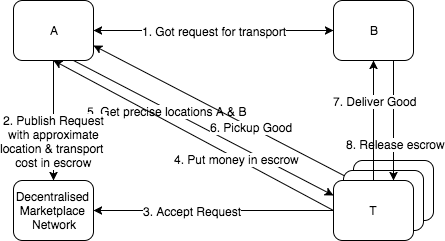
\includegraphics[scale=0.8]{hypothesis_actor_balance.png}
    \caption{Expected characteristic for intermediation}
\end{figure}

% Present a time line
% How will you validate your research?

% Required expertise for this project: Give a list of the expertise that is needed for the successful completion of this project. Examples are:
%   Java programming
%   Make and Makefiles
%   Configuration management
%   Testing
%   Etc., etc.
\section{Required expertise}

Languages
\begin{itemize}
    \item Python
    \item Solidity
    \item Go
\end{itemize}

\noindent Main
\begin{itemize}
    \item Make
    \item Git
    \item Dispersy (https://github.com/Tribler/dispersy message layer)
    \item PyQT (https://riverbankcomputing.com/software/pyqt/intro)
    \item NoseTest (http://nose.readthedocs.io/en/latest/)
    \item Package manager (pip)
    \item Yaml
    \item Docker
    \item IPFS
    \item Multi Signiture
    \item Ricardian Contracts
\end{itemize}

% Timeline: An overview of what activity will take place when, and what milestones/deadlines the project has.
\section{Timeline}

Timeline elements
\begin{itemize}
  \item Bootstrap dispersy/openbazaar
  \item Adjust bootstrapped platform shared protocol layer
  \item Create trustless intermediation logic
  \item Implement trustless intermediation
  \item Improve privacy
  \item Front-end
\end{itemize}

% Risks: Give an assessment of the risks for this project and present counter measures. These may include:
%   Project goals are too ambitious.
% The peer-to-peer logistics marketplace would connect demand and supply of supply chain logistics together. The demand side of logistics can be defined as actor A wanting to send goods to actor B, whereby the supply side is actor T willing to perform the transportation of goods along the supply chain. The main challenge with the execution of this relation is minimizing the trust which has to be put onto actor T and avoid the use of oracles to resolve dispute.\par
%   Project goals are too vague.
%   The information about the project is unavailable/incomplete/too difficult.
%   The gap between your expertise and the required expertise is too large
\section{Risks}
% The risk with the chosen research topic is that these p2p marketplace systems rely on trust mechanisms like reputation systems or a trustless public ledger. The reputation systems can be attacked with sybil attacks and the trustless idea of a public ledger can be argued that it is currently unachievable.\par
% If anonymity is not seen as a boolean value then the minimal situation of anonymity given to parties would be only the T knowing the location of actor A and actor B. The disclosure of the locations could be communicated only when actor T would already accepted the contract and is locked in to an escrow.

Assumptions to be taken beforehand:

\begin{itemize}
  \item Rational behaviour of actors
\end{itemize}

Limitations:

\begin{itemize}
  \item Transaction/conformation time blockchain
  \item What if end point is not available to receive transport?
\end{itemize}

% Literature survey (can also be a separate document): Describe the following for related scientific literature on your topic:
% Brief summary of contents,
% Relation to your topic: how does the work described in the reference differ from your approach, what results have they obtained, what open questions do they still have?
% A guideline is to include between 10 and 20 papers on your topic in the survey. The exact number depends on the topic and available literature.
\section{Literature survey}

\subsection{Trustless Intermediation in Blockchain-based Decentralized Service Marketplaces, 2017 \cite{trustlessIntermediationInBCServiceMarket}}
\textbf{Summary}: Service marketplaces promise an open platform for sellers and buyers of IT services. The marketplace design usually assumes that market functions, such as match-making, transaction settlement, and dis- pute resolution are performed by intermediaries in a centralized system. We propose the concept of trustless intermediation to enable new forms of decentralized service marketplaces. By leveraging blockchain-enabled smart contracts we eliminate the need for trust in marketplace interme- diaries and reduce barriers of entry, lock-in, and transaction costs, by removing now obsolete trust-establishing mechanisms. Desema, our de- centralized service marketplace prototype, is a first implementation of this concept that is based on the Ethereum blockchain in combination with IPFS, a peer-to-peer distributed file system.\newline
\textbf{Differ from my approach}: Klems et al., 2017 researched is towards trustless intermediation in decentralized service marketplaces whereby my research is aimed towards physical execution of transport. Due to it being in the physical domain other ways of making the process trustless need to be researched.\newline
\textbf{Obtained result}: Klems et al., 2017 created a prototype marketplace named Desema where they applied their trustless system architecture. \newline
\textbf{Remaining open questions}: Open challenges include the de- sign and development of more advanced and incentive-aligned approaches for trustless dispute resolution between service providers and consumers.\newline

\subsection{Beaver: A Decentralized Anonymous Marketplace with Secure Reputation, 2016 \cite{decentralizedAnonymousReputation}}
\textbf{Summary}: Amid growing concerns of government surveillance and corporate data sharing, web users increasingly demand tools for preserving their privacy without placing trust in a third party. Unfortunately, existing centralized reputation systems need to be trusted for either privacy, correctness, or both. Existing decentralized approaches, on the other hand, are either vulner- able to Sybil attacks, present inconsistent views of the network, or leak critical information about the actions of their users. In this paper, we present Beaver, a decentralized anonymous marketplace that is resistant against Sybil attacks on vendor reputation, while preserving user anonymity. Beaver allows its participants to enjoy open enrollment, and provides every user with the same global view of the reputation of other users through public ledger based consensus. Various cryptographic primitives allow Beaver to offer high levels of usability and practicality, along with strong anonymity guarantees. Operations such as creating a listing, purchasing an item, and leaving feedback take just milliseconds to compute and require generating just a few kilobytes of state while often constructing convenient anonymity sets of hundreds of transactions.\newline
\textbf{Differ from my approach}: Soska et al., 2016 offer an fully anonymous decentralized marketplace that is resistant against sybil attacks by leveraging costs against these actions. The reputation is actually registered on a blockchain which differs from my approach which does not aim for full anonymity and a mandatory registering of reputation in the blockchain. \newline
\textbf{Obtained result}: Soska et al., 2016 presented a decentralized anonymous marketplace with a incentive structure which counteracts the cost of Sybil attacks.\newline
\textbf{Remaining open questions}: Vendor privacy related to all transactions being anonymously stored on the blockchain, so the quantity of vendor transactions can be known. Unclaimed reviewing fees when customers do not follow the incentive structure. Customers deanonymizing themselves. Collusion attacks. Values of fees. \newline

\subsection{Building Trust in Decentralized Peer-to-Peer Electronic Communities, 2003 \cite{buildTrust}}
\textbf{Summary}: Many players in electronic markets have to cope with much higher amount of uncertainty as to quality and reliability of the products they buy and the information they obtain from other peers in the respective online business communities. One way to address this uncertainty problem is to use information such as feedbacks about past experiences to help making recommendation and judgment on product quality and information reliability. This paper presents PeerTrust, a simple yet effective reputation-based trust mechanism for quantifying and comparing the trustworthiness of peers in a decentralized peer-to-peer electronic marketplace. There are three main contributions in this paper. First, we argue that the trust models based solely on feedbacks from other peers in the community is inaccurate and ineffective. We introduce three basic trust parameters in computing trust within an electronic community. In addition to feedbacks in terms of amount of satisfaction, we incorporate the feedback context such as the total number of transactions and the credibility of the feedback sources into the PeerTrust model for evaluating the trustworthiness of peers. Second, we develop a basic trust metric that combines the three critical parameters to compare and quantify the trustworthiness of peers. Third, we present a concrete method to validate the proposed trust model and report the set of initial experiments, showing the feasibility, costs, and benefits of our approach.\newline
\textbf{Differ from my approach}: Xiong \& Liu, 2003 focus on the wide domain of trust in decentralized peer-to-peer communities. With my specific case regarding a marketplace with transport of goods trust between the peers is an important aspect but is more contained in a specific domain than Xiong \& Liu.\newline
\textbf{Obtained result}: Xiong \& Liu, 2003 present PeerTrust a trust mechanism for building trust in peer-to-peer electronic communities. They identified three important trust parameters, these are: amount of satisfaction, number of interactions and balance factor of trust. They put the results into experiments which demonstrated the effectiveness, costs, and benefits of the approach.\newline
\textbf{Remaining open questions}: Looking at ways to make the approach more robust against malicious behaviors, such as collusions among peers. Combining trust management with intrusion detection to address concerns of sudden and malicious attacks. How to uniquely identify peers over time and associate their histories with them\newline

\subsection{Reputation Systems for Anonymous Networks, 2008 \cite{reputationSystemAnonymous}}
\textbf{Summary}: We present a reputation scheme for a pseudonymous peer-to-peer (P2P) system in an anonymous network. Misbehavior is one of the biggest problems in pseudonymous P2P systems, where there is little incentive for proper behavior. In our scheme, using ecash for reputation points, the reputation of each user is closely related to his real identity rather than to his current pseudonym. Thus, our scheme allows an honest user to switch to a new pseudonym keeping his good reputation, while hindering a malicious user from erasing his trail of evil deeds with a new pseudonym.\newline
\textbf{Differ from my approach}: The reputation system is organized through a central entity called bank which is responsible for the reputation value exchange by the means of coins. This centralizes the reputation system which differs from my approach. \newline
\textbf{Obtained result}: The first contribution is defining security for identity bound reputation systems. The second contribution is the constriuction of a raputation scheme that satisfies the security definition.\newline
\textbf{Remaining open questions}: First, the scheme uses unit coins for reputation whereby the coins have variable value while constant value is preferable. Secondly, negative feedback is not possible to generate. Finally, getting rid of the bank which is a trusted entity to maintain reputation balance correctly.\newline

\subsection{Decentral Market Self-regulating electronic market, 2016 \cite{decentralMarket}}
\textbf{Summary}: A decentral electronic marketplace to trade digital currencies was created for this project. Users may trade MultiChain balance for Bitcoin. MultiChain can be described as up- and download currency in a peer-to-peer network. When a peer uploads, the balance of that peer increases and the peer can download more effectively. The client for this project is the Tribler Team. Most of the Tribler Team’s work revolves around Tribler: an open-source peer-to-peer program which enables its users to find, enjoy, and share content. An earlier bachelor end-project implemented a partial, functional prototype of this idea. We improved the existing concepts and re-implemented a decentralised market from scratch with scalability and as much security as possible, given the limited available development time. This market is the first electronic marketplace to be fully decentralized. There were previous attempts to create such a marketplace, but those implementations fell short in scalability and security. During the research phase, we discovered that the previous decentral market project was not scalable and not production ready, so we made the decision to, together with our client, instead build our application upon a more production-level network platform known as Dispersy. As nothing on the Internet can be trusted which is a problem on its own, we could not make the product as secure as we would have wanted to. At a technical level our contribution consists of 7000+ lines of code, 50+ test suites with a code coverage of +95\% and documentation for Dispersy.\newline
\textbf{Differ from my approach}: Decentralized market for currency exchange whereby my approach uses a different network platform and use case.\newline
\textbf{Obtained result}: A decentral electronic marketplace to trade digital currencies.\newline
\textbf{Remaining open questions}: How to create a fitting trust system? How to not have a NAT between the peers? \newline

\subsection{The challenge of decentralized marketplaces, 2017 \cite{challangeDecentralizedMarketplaces}}
\textbf{Summary}: Online trust systems are playing an important role in to-days world and face various challenges in building them. Billions of dollars of products and services are traded through elec- tronic commerce, files are shared among large peer-to-peer networks and smart contracts can potentially replace pa- per contracts with digital contracts. These systems rely on trust mechanisms in peer-to-peer networks like reputation systems or a trustless public ledger. In most cases, reputa- tion systems are build to determine the trustworthiness of users and to provide incentives for users to make a fair con- tribution to the peer-to-peer network. The main challenges are how to set up a good trust system, how to deal with se- curity issues and how to deal with strategic users trying to cheat on the system. The Sybil attack, the most important attack on reputation systems is discussed. At last match making in two sided markets and the strategy proofness of these markets are discussed.\newline
\textbf{Differ from my approach}: Very similair by giving a rundown of all the research done towards trust enforcements in p2p file sharing, decentralized markets and sybil attacks. \newline
\textbf{Obtained result}: B van Ijzendoorn gives a summary of academical research on decentralization, Sybil attacks, trust and peer-to-peer in relation to marketplaces. \newline
\textbf{Remaining open questions}: Not applied.\newline

\subsection{A Peer-To-Peer Platform for Decentralized Logistics, 2017 \cite{peer-to-peerDecentralizedLogistics}}
\textbf{Summary}: We introduce a novel platform for decentralized logistics, the aim of which is to magnify and accelerate the impact o ered by the integration of the most recent advances in Information and Communication Technologies (ICTs) to multi-modal freight operations. The essence of our peer-to-peer (P2P) framework distributes the management of the logistics operations to the multiple actors according to their available computational resources. As a result, this new approach prevents the dominant players from capturing the market, ensures equal opportunities for di erent size actors, and avoids vendor lock-in. The latest ICTs such as In- dustrial Data Space (IDS), Blockchain, and Internet-of-Things (IoT) are used as basic building blocks which, together, enable the creation of a trusted and inte- grated platform to manage logistics operations in a fully decentralized way. While IDS technology allows for secured data exchange between the di erent parties in the logistics chain, Blockchain technology handles transaction history and agreements between parties in a decentralized way. IoT enables the gathering of real-time data over the logistics network, which can be securely exchanged between the di erent parties and used for managing the decision-making related to the control of the freight transportation activities. The practicability and the potential of the proposed platform is demonstrated with two use cases, involving various actors in the logistics chains.\newline
\textbf{Differ from my approach}: It is an academic research which originated from the logistics domain and aimed at solving the contradiction between interoperability and data sovereignty.\newline
\textbf{Obtained result}: High level decentralized logistics system architecture with data flows. Two initial use cases.\newline
\textbf{Remaining open questions}: Development of business models in parallel.\newline

\subsection{The Concept Of Decentralized And Secure Electronic Marketplace, 2008 \cite{Serban2008}}
\textbf{Summary}: For commerce (electronic or traditional) to be effective, there must be a degree of trust between buyers and sellers. In traditional commerce, this kind of trust is based on such things as societal laws and customs, and on the intuition people tend to develop about each other during interpersonal interactions. The trustworthiness of these factors is based, to a large extent, on the geographical proximity between buyers and sellers. But this proximity is lost in e-commerce. In conventional electronic marketplaces the trust among participants is supported by a central server which imposes certain trading rules on all transactions. But such centralized marketplaces have serious drawbacks, among them: lack of scalability, and high cost. In this paper we propose the concept of Decentralized Electronic Marketplace (DEM) which allow buyers and sellers to engage in commercial transactions, subject to an explicitly stated set of trading rules, called the law of this marketplace — which they can trust to be observed by their trading partners. This trust is due to a decentralized, and thus scalable, mechanism that enforces the stated law of the DEM. We implement an electronic marketplace for airline tickets in order to illustrate the feasibility of the proposed concepts for decentralized and secure electronic marketplace.\newline
\textbf{Differ from my approach}: Defined roles with clear identification needed to fulfill them. Different use case being fulfilled by the marketplace.\newline
\textbf{Obtained result}: Concept of Decentralized Electronic Marketplace (DEM) implemented with airline tickets.\newline
\textbf{Remaining open questions}: Who is the responsible for deciding if a actor is fit to fulfill a role on the network?\newline

\subsection{Building an E-Marketplace on a Peer-to-Peer Infrastructure, 2004 \cite{buildingp2pmarketplace}}
\textbf{Summary}: Existing e-marketplaces, built on traditional client-server architectures, severely restrict the scope and dynamics of Business-to-Business (B2B) interactions. Peer-to-peer (P2P) architectures will provide far more decentralised infrastructures, while allowing a much wider range of business patterns to take place. On one hand, the interaction over a P2P network resembles the way real-world enterprises perform business with each other. On the other hand, a small set of simple services is enough to support complex business processes over a P2P infrastructure. Incidentally, most of the required technology is readily available, though it may be necessary to bring in an appropriate integration of different concepts. The paper discusses the implementation of essential services for P2P e-marketplaces, based on one of the leading P2P platforms, and illustrates its benefits by applying the P2P approach to a vendor of industrial equipment.\newline
\textbf{Differ from my approach}: Due to the paper being fairly out dates the  project JXTA being used as a peer-to-peer platform for the research is outdated. Currently the best foundation for Bootstrapping an peer-to-peer marketplace is Openbazaar or Dispersy. The research also focuses on shifting b2b to p2p which differs from my research.\newline
\textbf{Obtained result}: Discusses the implementation of essential services for peer-to-peer marketplaces, based on one of the leading peer-to-peer platforms, and illustrates its benefits from a vendors perspective.\newline
\textbf{Remaining open questions}: Advances in e-contracting and trading partner agreements are necessary in order to establish some standardized approaches in the area. This is exactly what i will be researching regarding logistics. \newline

\bibliographystyle{plain}
\bibliography{papers}

\end{document}
